\chapter{Ideas and concepts}
\label{ch:Ideas-Concepts}

In this chapter, the various ideas and concepts used in the thesis are discussed in more detail. It includes pieces of information about the dataset used in section \ref{sec:Dataset}, the default architecture and the training of the models.

\section{Problem definition}
\label{sec:Problem-Definition}

\section{Concluding problem definition}
\label{sec:Concluding-Problem-Definition}

\section{Dataset}
\label{sec:Dataset}
This section introduces the dataset used in the project, and as well as explains the underlying data structure. The section \ref{sub:SINS-Database} introduces the \gls{SINS} database. And the subsequent section \ref{sub:DCASE-Task-Dataset} introduces a reduced derivation of the \gls{SINS} database, which is the primary dataset used for the project.

\subsection{SINS Database}
\label{sub:SINS-Database}
The \gls{SINS} database is a publicly available dataset developed to improve models used for \gls{AAL}. In \gls{AAL} persons are monitored, e.g. to support patients with a chronic illness and older persons, by tracking their activities being performed at home.
\newline
\newline
The paper \cite{dekkers_sins_2017} introduces the \gls{SINS} database, which contains recordings of one living home, over a period of one week. The home consisted of five different rooms: a combined living room and kitchen, bathroom, toilet, bedroom and hall. In each one of these rooms, one or more sensor nodes, each containing four linearly arranged microphones which were uniformly distributed as indicated by figure \ref{fig:sins-database-floor-map}.

\begin{figure}[H]
	\centering
	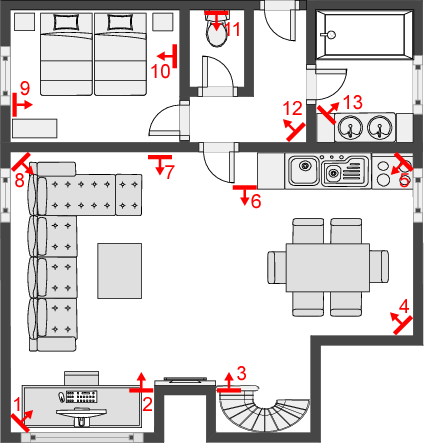
\includegraphics[scale=0.3]{baa-documentation/img/SINS_database_floor_map.png}
	\caption[SINS database recording environment map]{SINS database recording environment map \footnotemark}
	\label{fig:sins-database-floor-map}
\end{figure}
\footnotetext{\href{https://www.semanticscholar.org/paper/THE-SINS-DATABASE-FOR-DETECTION-OF-DAILY-ACTIVITIES-Dekkers-Lauwereins/de84995b6b0042c9f6f1ccbd1f13d75b14c24e80/figure/1}{\nolinkurl{semanticscholar.org/paper/THE-SINS-DATABASE-FOR-DETECTION-OF-DAILY-ACTIVITIES-Dekkers-Lauwereins}}}

One person lived in the environment for a continuous duration of one week. In order to have an as realistic as possible data recording, there was no predefined set of scenarios. Due to that, the recorded activities also included being absent from the home. Although there were no restrictions on the actions, the number of activities that were labelled was limited, as indicated in figure \ref{fig:sins-database-recorded-activities}. In total there are 16 different recorded activities in five different rooms. Figure \ref{fig:sins-database-recorded-activities} lists the different activities along with the number of examples and the mean and standard deviation and the duration of all examples for each room.

\begin{figure}[H]
	\centering
	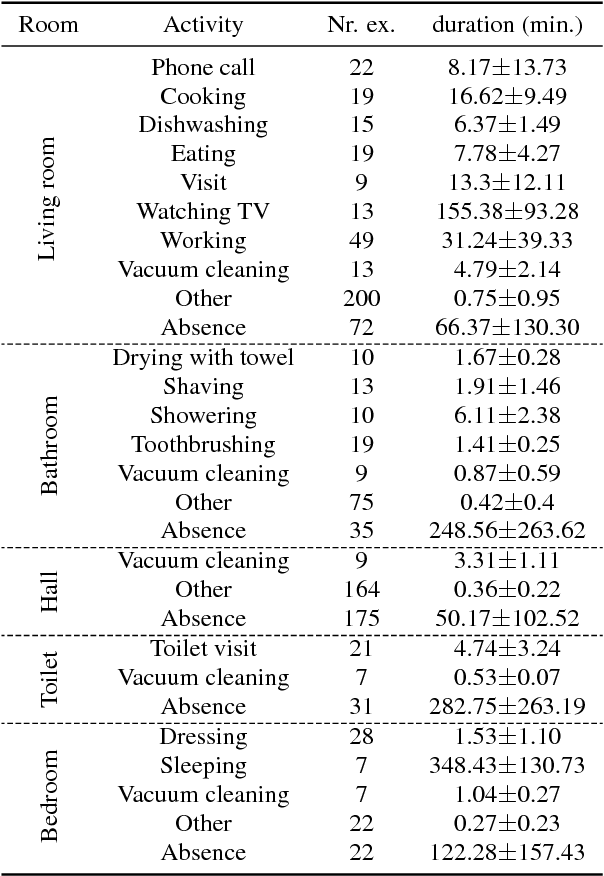
\includegraphics[scale=0.3]{baa-documentation/img/SINS_database_recorded_activities.png}
	\caption[SINS database recorded activities]{SINS database recorded activities \footnotemark}
	\label{fig:sins-database-recorded-activities}
\end{figure}
\footnotetext{\href{https://www.semanticscholar.org/paper/THE-SINS-DATABASE-FOR-DETECTION-OF-DAILY-ACTIVITIES-Dekkers-Lauwereins/de84995b6b0042c9f6f1ccbd1f13d75b14c24e80/figure/1}{\nolinkurl{semanticscholar.org/paper/THE-SINS-DATABASE-FOR-DETECTION-OF-DAILY-ACTIVITIES-Dekkers-Lauwereins}}}

\subsection[DCASE 2018 Challenge - Task 5]{DCASE 2018 Challenge - Task 5: Monitoring of domestic activities based on multi-channel acoustics \footfullcite{dekkers_sins_2017}}
\label{sub:DCASE-Task-Dataset}
This resource contains all the necessary information about the challenge from the IEEE AASP Challenge on \gls{DCASE} 2018. The challenge finished in 2018, and the results, as well as the full dataset, were published. The main goal of the challenge was to classify multi-channel audio segments into predefined classes and determine how beneficial multi-channel recordings are for classification. 

\begin{figure}[H]
	\centering
	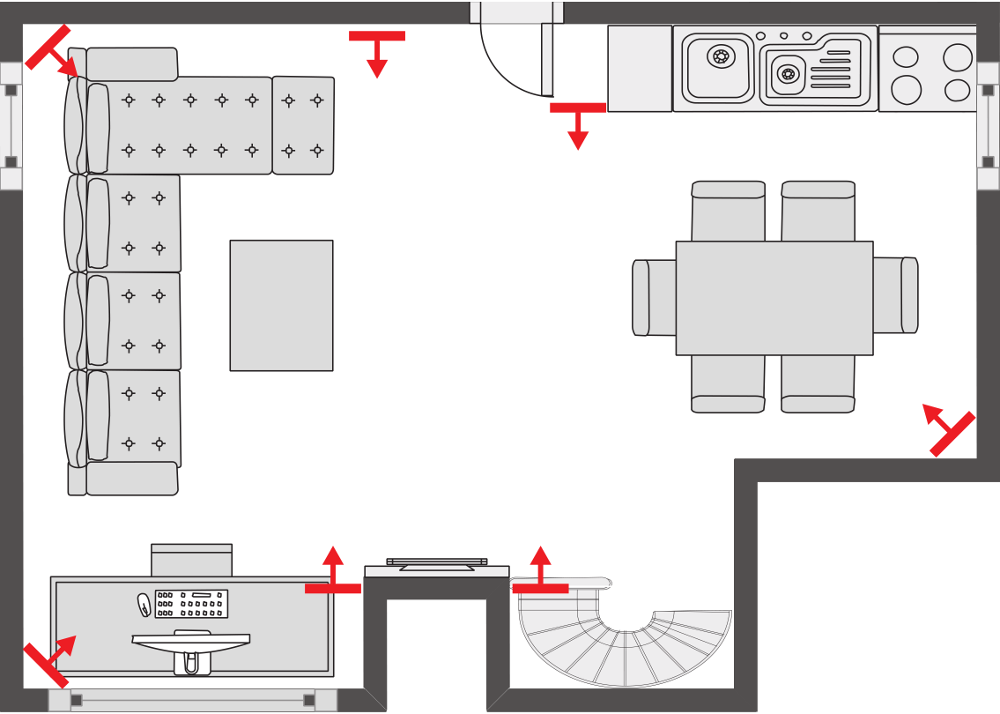
\includegraphics[scale=0.8]{baa-documentation/img/DCASE_floor_map.png}
	\caption[2D floor plan of the combined kitchen and living room with the used sensor nodes]{2D floor plan of the combined kitchen and living room with the used sensor nodes \footnotemark}
	\label{fig:dcase-recordings-floor-plan}
\end{figure}
\footnotetext{\href{http://dcase.community/challenge2018/task-monitoring-domestic-activities}{\nolinkurl{dcase.community/challenge2018/task-monitoring-domestic-activities}}}

The dataset used in the challenge is an abbreviation of the \nameref{sub:SINS-Database}; where only seven of the thirteen microphone nodes were considered. These nodes are from the room combination from the living room and the kitchen, as illustrated in figure \ref{fig:dcase-recordings-floor-plan}. Every recording of an activity is split into ten-second recordings, which are called segments. Every segment has four channels which correspond to the four different microphone channels of each node. Within the dataset, there are no overlapping sounds, from actions performed simultaneously. That means that every segment has an activity label assigned to it. There are a total of nine different activity labels, which all refer to a daily activity performed at home.

\begin{table}[H]
    \centering
    \caption[Activities performed in the dataset proposed by DCASE]{Activities performed in the dataset proposed by DCASE \footnotemark}
	\label{tab:DCASE-activiies-performed}
    \begin{tabular}{l|l|l}
        \toprule
        \textbf{Activity performed} & \textbf{\# 10s segments} & \textbf{\# sessions} \\ 
        \midrule[1pt]
        Absence (nobody present in the room) & 18860 & 42 \\
        \hline
        Cooking & 5124 & 13 \\ 
        \hline
        Dish washing & 1424 & 10 \\ 
        \hline
        Eating & 2308 & 13 \\ 
        \hline
        Other (present, but not doing any relevant activity) & 2060 & 118 \\ 
        \hline
        Social activity (visit, phone call, ...) & 4944 & 21 \\ 
        \hline
        Vacuum cleaning & 972 & 9 \\ 
        \hline
        Watching TV & 18648 & 9 \\ 
        \hline
        Working (typing, mouse clicking, ...) & 18644 & 33 \\ 
        \midrule[1pt]
        \textbf{Total} & \textbf{72984} & \textbf{268} \\
        \bottomrule
    \end{tabular}
\end{table}
\footnotetext{\href{http://dcase.community/challenge2018/task-monitoring-domestic-activities}{\nolinkurl{dcase.community/challenge2018/task-monitoring-domestic-activities}}}

In the challenge, the data was split into a development and an evaluation set. The development set is used for training the model and was made available for everyone participating in the challenge. It contains four of the seven microphone nodes which are 200h of audio data. This dataset also contains the corresponding label to each audio segment. The evaluation set is used for evaluating the final models to see their performance on never seen before data from the other three nodes. A session of an activity is a full recording of an action. Within both of these datasets, each session was kept together.

\section{Current research}
\label{sec:Current-Research}

\subsection{Training environment}
\label{sub:Training-Environment}
